\part{Object-Oriented Programming (2/2)}
\label{part:oop2}

\section{Object-Oriented Programming -- Inheritance, Polymorphism, Idioms}

\subsection{Inheritance}

\subsubsection{Derived classes}

% Source: https://en.cppreference.com/w/cpp/language/derived_class
\begin{frame}{Derived Classes}{}
  \begin{block}{Derived Classes}
    Any class may be declared as \emph{derived} from one or more \emph{base classes} which, in turn, may be derived from their own base classes, forming an inheritance hierarchy. Each base class:
    \begin{itemize}
    \item
      may have an access specifer: \lstinline!public!, \lstinline!protected!, \lstinline!private!
    \item
      may be declared \lstinline!virtual!
    \end{itemize}
  \end{block}

  \begin{block}{Remark}
    If the access specifier is omitted, it defaults to:
    \begin{itemize}
    \item
      \lstinline!public! for \lstinline!struct!
    \item
      \lstinline!private! for \lstinline!class!
    \end{itemize}
  \end{block}
\end{frame}

\begin{frame}{Derived Classes}{}
  \begin{example}[Derived Classes]
    \sourceinput{snippets/derived_class.cc}
  \end{example}
\end{frame}


\begin{frame}{Inheritance and member access}{}
  \begin{block}{Inheritance and member access}
    \begin{center}
      \lstinline[mathescape]!struct B \{ \}; struct D : $\;specifier\;$ B \{ \};!

      \bigskip

      \begin{tabular}{|c|c|c|c|}
      \hline
      Inheritance           & \multicolumn{3}{|c|}{Member in \lstinline!B!} \\
      \lstinline[mathescape]!$specifier$! & \lstinline!public!    & \lstinline!protected! & \lstinline!private! \\
      \hline
      \lstinline!public!    & \lstinline!public!    & \lstinline!protected! & - \\
      \lstinline!protected! & \lstinline!protected! & \lstinline!protected! & - \\
      \lstinline!private!   & \lstinline!private!   & \lstinline!private!   & - \\
      \hline
      \end{tabular}

      Member access in \lstinline!D!
    \end{center}
  \end{block}
\end{frame}

\subsubsection{Virtual base classes}

% Source: https://en.cppreference.com/w/cpp/language/derived_class
\begin{frame}{Virtual base class}{}
  \begin{block}{Virtual base class}
    For each distinct base class that is specified \lstinline!virtual!, the most derived object contains only one base class subobject of that type, even if the class appears many times in the inheritance hierarchy (as long as it is inherited \lstinline!virtual! every time).
  \end{block}

  \begin{example}[Famous example of virtual base class]
    \begin{center}
    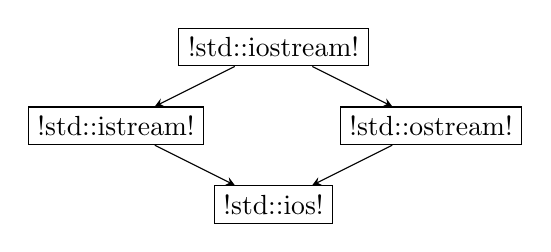
\begin{tikzpicture}
      \node[draw] (IO) at ( 0, 0) { \lstinline!std::iostream! } ;
      \node[draw] (I) at (-2,-1) { \lstinline!std::istream! } ;
      \node[draw] (O) at ( 2,-1) { \lstinline!std::ostream! } ;
      \node[draw] (B) at ( 0,-2) { \lstinline!std::ios! } ;

      \draw[->,>=stealth] (IO) -- (I) ;
      \draw[->,>=stealth] (IO) -- (O) ;
      \draw[->,>=stealth] (I) -- (B) ;
      \draw[->,>=stealth] (O) -- (B) ;
    \end{tikzpicture}
    \end{center}
  \end{example}
\end{frame}

\begin{frame}{Virtual base class}{}
  \begin{example}[Virtual base class]
    \sourceinput{snippets/virtual_base_class.cc}
  \end{example}
\end{frame}

% TODO: initialization of virtual base class?


\subsubsection{Empty Base Optimization (EBO)}

% Source: https://en.cppreference.com/w/cpp/language/ebo
\begin{frame}{Empty Base Optimization (EBO)}{}
  \begin{block}{Empty Base Optimization (EBO)}
    \strong{Empty Base Optimization} (EBO) allows the size of an empty base subobject to be zero
  \end{block}

  \begin{block}{Explanation}
    \begin{itemize}
    \item
      The size of any object or member subobject is required to be at least 1 even if the type is an empty class, in order to be able to guarantee that the addresses of distinct objects of the same type are always distinct.
    \item
      However, base class subobjects are not so constrained, and can be completely optimized out from the object layout
    \end{itemize}
  \end{block}
\end{frame}

\begin{frame}{Empty Base Optimization}{}
  \begin{example}[Empty Base Optimization]
    \sourceinput{snippets/ebo.cc}
  \end{example}
\end{frame}


\subsection{Polymorphism}

\subsubsection{Virtual functions}

% Source: https://en.cppreference.com/w/cpp/language/virtual
\begin{frame}{Virtual functions}{}
  \begin{definition}[Virtual function]
    A \strong{virtual function} is a non-static member function with the \lstinline!virtual! specifier. A virtual function supports dynamic dispatch, i.e. its behavior can be overridden in derived classes.
  \end{definition}

  \begin{block}{Virtual functions override}
    A function that overrides a virtual function in a derived class must have the same:
    \begin{itemize}
    \item
      name
    \item
      parameter type list (but not the return type)
    \item
      cv-qualifiers and ref qualifiers
    \end{itemize}
  \end{block}

  \begin{block}{Remark}
    A virtual function does not need to be visible (\lstinline!public! or \lstinline!protected!) to be overridden.
  \end{block}
\end{frame}

\begin{frame}{Virtual functions}{}
  \begin{example}[Virtual functions]
    \sourceinput{snippets/virtual_functions.cc}
  \end{example}
\end{frame}

% Source: https://en.cppreference.com/w/cpp/language/virtual
\begin{frame}{\texttt{override} and \texttt{final}}{}
  \begin{block}{\texttt{override} and \texttt{final}}
    \begin{itemize}
    \item
      If a function is declared with the specifier \lstinline!override!, but does not override a virtual function, the program is ill-formed
    \item
      If a function is declared with the specifier \lstinline!final!, and another function attempts to override it, the program is ill-formed
    \end{itemize}
  \end{block}
\end{frame}

\begin{frame}{\texttt{override} and \texttt{final}}{}
  \begin{example}[\texttt{override} and \texttt{final}]
    \sourceinput{snippets/override_and_final.cc}
  \end{example}
\end{frame}

\subsubsection{Virtual destructors}

% Source: https://en.cppreference.com/w/cpp/language/virtual
\begin{frame}{Virtual destructor}{}
  \begin{block}{Virtual destructor}
    Even though destructors are not inherited, if a base class declares its destructor virtual, the derived destructor always overrides it. This makes it possible to delete dynamically allocated objects of polymorphic type through pointers to base.
  \end{block}
  \begin{block}{Important remark}
    If a class is polymorphic (declares or inherits at least one virtual function), it must declare its destructor \lstinline!virtual!.
  \end{block}
\end{frame}

\begin{frame}{Virtual destructor}{}
  \begin{example}[Virtual destructor]
    \sourceinput{snippets/virtual_destructor.cc}
  \end{example}
\end{frame}

\subsubsection{Pure virtual functions}

% Source: https://en.cppreference.com/w/cpp/language/abstract_class
\begin{frame}{Pure virtual functions and abstract classes}{}
  \begin{definition}[Pure virtual function]
    A \strong{pure virtual function} is a virtual function with the \emph{pure specifier} noted \lstinline!= 0!.
  \end{definition}

  \begin{definition}[Abstract class]
    An \strong{abstract class} is a class that either defines or inherits at least one pure virtual function.
  \end{definition}

  \begin{block}{Remarks}
    \begin{itemize}
    \item
      No objects of an abstract class can be created
    \item
      Abstract classes are used as base classes for concrete classes
    \end{itemize}
  \end{block}
\end{frame}

\begin{frame}{Pure virtual functions and abstract classes}{}
  \begin{example}[Abstract class]
    \sourceinput{snippets/abstract_class.cc}
  \end{example}
\end{frame}

\subsubsection{Virtual table}

% Source: https://en.wikipedia.org/wiki/Virtual_method_table
\begin{frame}{Virtual table and virtual table pointer}{}
  \begin{definition}[Virtual table]
    A \strong{virtual table} (or vtable) is a per-class table containing function pointers to virtual functions. It is generated by the compiler.
  \end{definition}

  \begin{definition}[Virtual table pointer]
    A \strong{virtual table pointer} (or vptr) is a per-object pointer to a virtual table added by the constructor. The vptr is part of the object.
  \end{definition}

  \begin{block}{Call to a virtual function}
    \begin{enumerate}
    \item
      Fetch the virtual table pointer of the object
    \item
      Call the function declared in the table pointed by the virtual table pointer
    \end{enumerate}
    Consequence: calling a virtual function requires an indirection!
  \end{block}
\end{frame}

\begin{frame}{Virtual table and virtual table pointer}{}
  \begin{example}[Virtual table and virtual table pointer]
    \sourceinput{snippets/vtable_vptr.cc}
  \end{example}
\end{frame}

\subsubsection{Run-time type information (RTTI)}

% Source: https://en.cppreference.com/w/cpp/language/dynamic_cast
\begin{frame}{\texttt{dynamic\_cast}}{}
  \begin{block}{\texttt{dynamic\_cast}}
    A \strong{\lstinline!dynamic_cast!} safely converts pointers and references to classes up, down, and sideways along the inheritance hierarchy.

    {
      \hfill\lstinline[mathescape]!dynamic_cast<$type$>($expr$)!\hfill
    }

    \lstinline[mathescape]!$expr$! is:
    \begin{itemize}
    \item
      A glvalue of a complete class type if \lstinline[mathescape]!$type$! is a reference
    \item
      A prvalue of a pointer to a complete class type if \lstinline[mathescape]!$type$! is a pointer
    \end{itemize}
  \end{block}

  \begin{block}{Result of a \texttt{dynamic\_cast}}
    \begin{itemize}
    \item
      If the cast is successful, \lstinline!dynamic_cast! returns a value of type \lstinline[mathescape]!$type$!.
    \item
      If the cast fails and \lstinline[mathescape]!$type$! is a pointer type, it returns a null pointer.
    \item
      If the cast fails and \lstinline[mathescape]!$type$! is a reference type, it throws an exception that matches a handler of type \lstinline!std::bad_cast!.
    \end{itemize}
  \end{block}
\end{frame}

\begin{frame}{\texttt{dynamic\_cast}}{}
  \begin{example}[\texttt{dynamic\_cast}]
    \sourceinput{snippets/dynamic_cast.cc}
  \end{example}
\end{frame}

% Source: https://en.cppreference.com/w/cpp/language/typeid
\begin{frame}{\texttt{typeid}}{}
  \begin{block}{\texttt{typeid}}
    The \lstinline!typeid! operator queries information of a type and returns an object of type \lstinline!const std::type_info&!. It can be used:
    \begin{itemize}
    \item
      with a type
    \item
      with an expression
    \end{itemize}
  \end{block}

  \begin{block}{\texttt{typeid} with an expression}
    \begin{itemize}
    \item
      If the expression is a glvalue expression that identifies an object of a polymorphic type, the \lstinline!typeid! expression evaluates the expression and then refers to the \lstinline!std::type_info! object that represents the dynamic type of the expression
    \item
      If expression is not a glvalue expression of polymorphic type, \lstinline!typeid! does not evaluate the expression, and the \lstinline!std::type_info! object it identifies represents the static type of the expression
    \end{itemize}
  \end{block}
\end{frame}

\begin{frame}{\texttt{typeid}}{}
  \begin{example}[\texttt{typeid}]
    \sourceinput{snippets/typeid.cc}
  \end{example}
\end{frame}

\subsection{Idioms}

\subsubsection{PImpl My Ride}

% Source: https://en.cppreference.com/w/cpp/language/pimpl
% Source: https://cpppatterns.com/patterns/pimpl.html
% Source: https://wiki.qt.io/D-Pointer
\begin{frame}{PImpl: Pointer to Implementation}{}
  \begin{block}{PImpl: Pointer to Implementation}
    \strong{PImpl} (Pointer to Implementation) (a.k.a. d-pointer or opaque pointer) is a technique to hide implementation details of a class in order to achieve ABI stability.
  \end{block}

  \begin{block}{PImpl in practice}
    \sourceinput{snippets/pimpl.cc}
  \end{block}
\end{frame}

\begin{frame}{PImpl or not PImpl}{}
  \begin{block}{Advantages of PImpl}
    \begin{itemize}
    \item
      Compilation firewall: a modification in \lstinline!Impl! does not require a recompilation of all classes that use \lstinline!Foo!
    \item
      Move-friendly: a \lstinline!std::unique_ptr! is easy to move, especially in containers
    \end{itemize}
  \end{block}
  \begin{block}{Drawbacks of PImpl}
    \begin{itemize}
    \item
      Access overhead: an access to a member requires an indirection through a pointer
    \item
      Space overhead: the object requires an additional pointer
    \item
      Lifetime management: the implementation object is allocated on the heap
    \item
      Maintenance overhead: all the implementation has to be in a dedicated file
    \end{itemize}
  \end{block}
\end{frame}


\subsubsection{\texttt{const} correctness}

% Source: https://isocpp.org/wiki/faq/const-correctness
\begin{frame}{\texttt{const} correctness}{}
  \begin{block}{\texttt{const} correctness}
    \lstinline!const! correctness is a set of rules to offer a guarantee about the (non-)mutability of object:
    \begin{itemize}
    \item
      Choose reference to \lstinline!const! or pointer to \lstinline!const! for parameters if you do not intend to modify the parameters
    \item
      Make a member function \lstinline!const! if the function does not modify the object
    \item
      If a member function is \lstinline!const! and returns a reference to a member, the reference should be \lstinline!const! or the function should return by value
    \end{itemize}
  \end{block}

  \begin{block}{Benefits of \texttt{const} correctness}
    \begin{itemize}
    \item
      The caller has the guarantee that a variable or an object will not be modified
    \item
      The compiler ensures that the callee respects the contract by emitting an error in case of modification of a \lstinline!const! object
    \item
      The \lstinline!const! property is spread through member function calls
    \end{itemize}
  \end{block}
\end{frame}

% overload const/non-const
\begin{frame}{\texttt{const} correctness}{}
  \begin{example}[\texttt{const} correctness]
    \sourceinput{snippets/const_correctness.cc}
  \end{example}
\end{frame}



% (N)RVO
